
    \section{max(G,S)}
    \import{latex_files/}{table_5.tex}

    \begin{figure}[H] % Pour insérer une figure
        \centering % Pour centrer l'image
        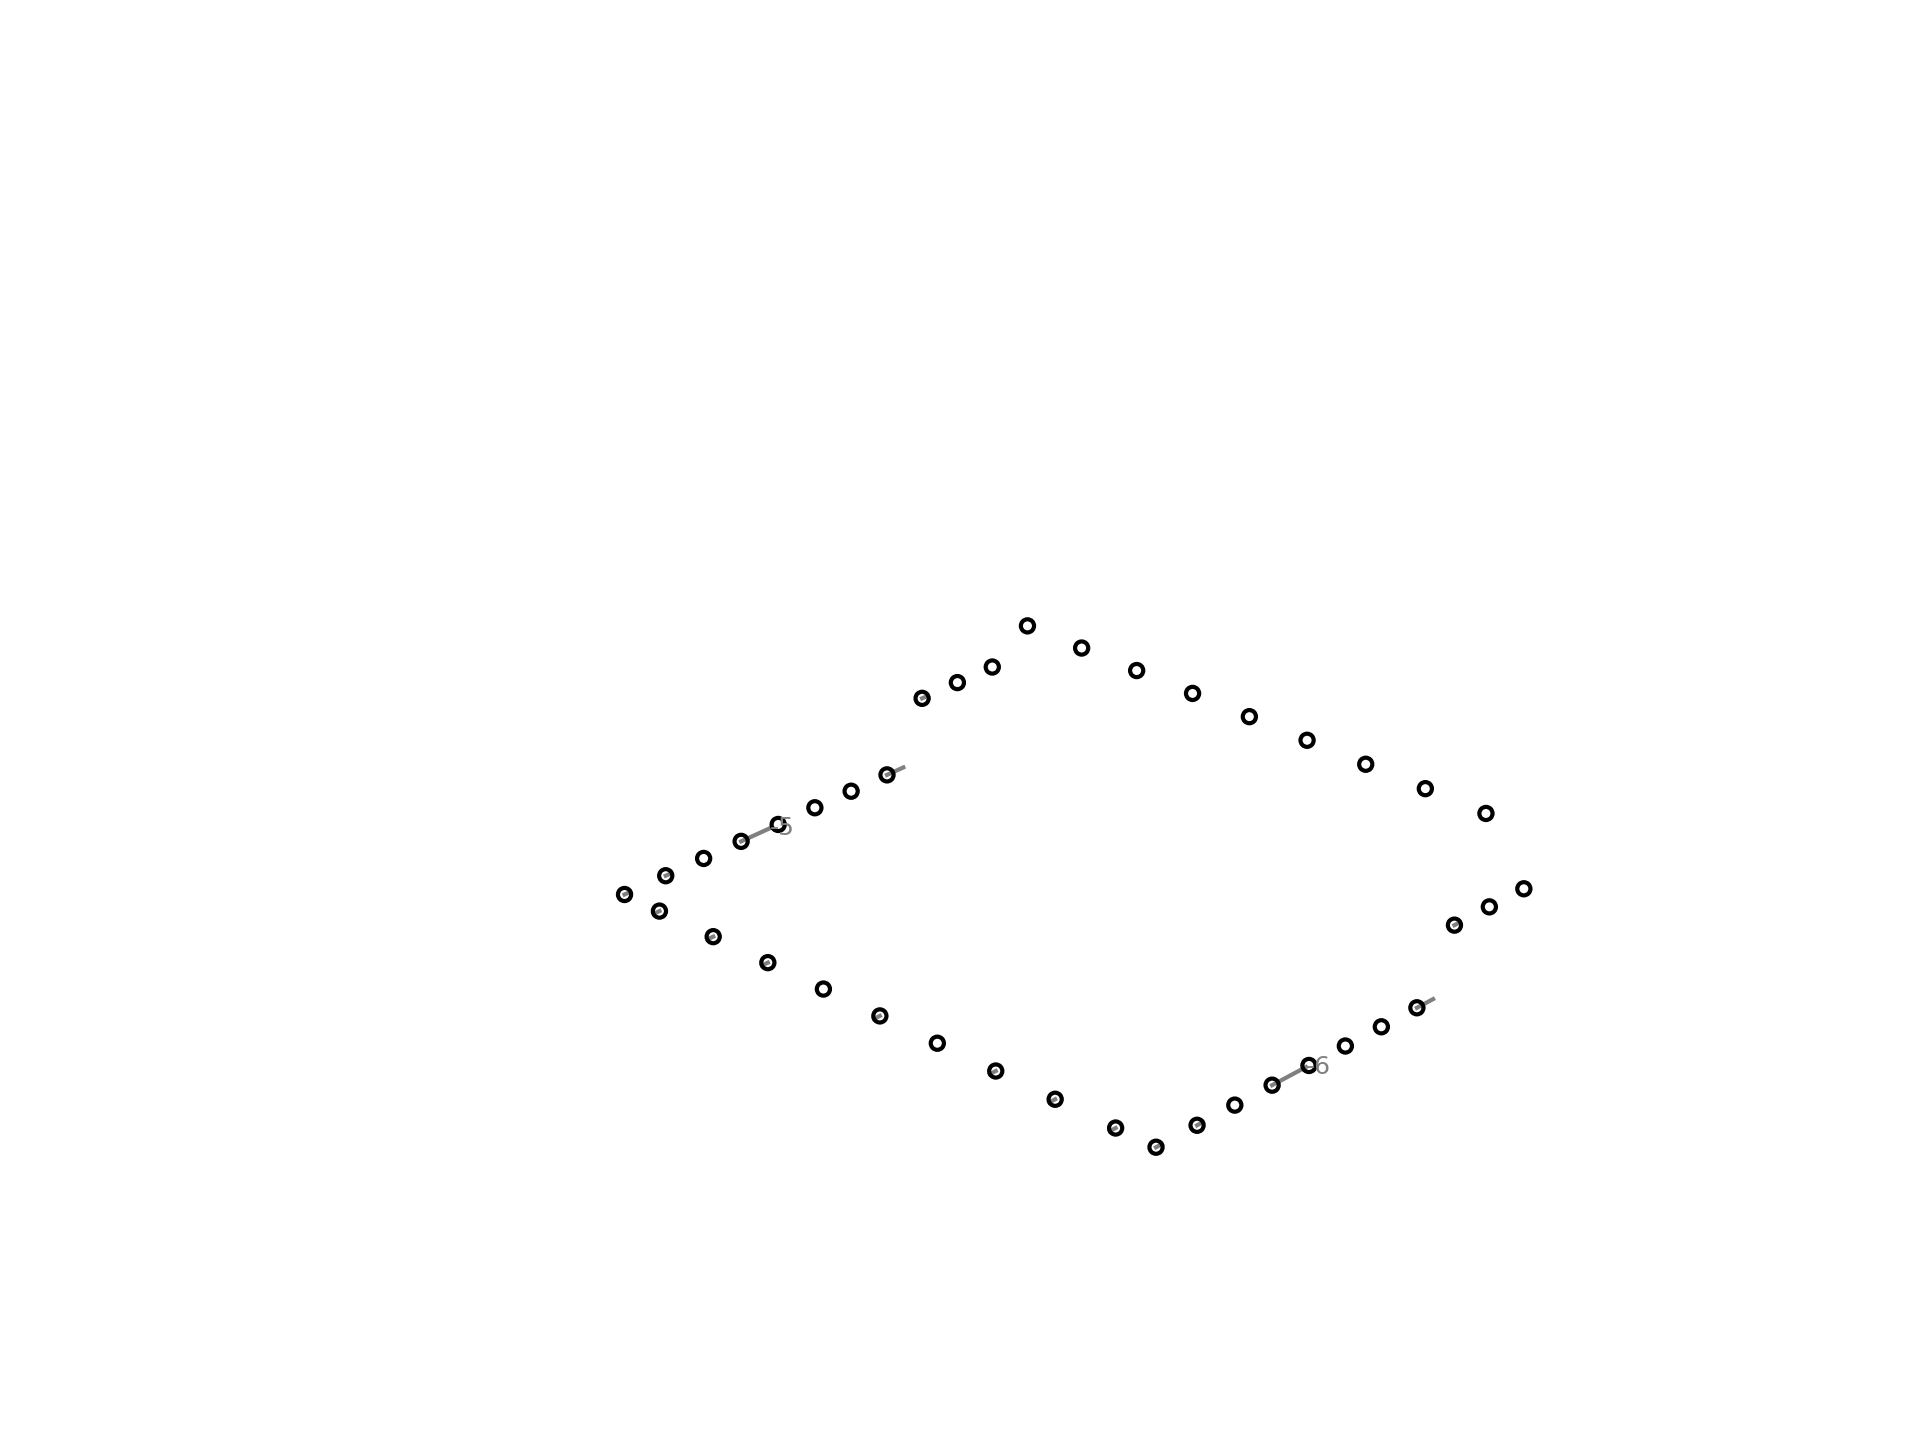
\includegraphics[width=\textwidth]{assets/img/graph3D_charges_cas_5_RFx_kN.png} % Pour insérer l'image
        \caption{max(G,S)\_RFx\_kN} % Légende de l'image
    \end{figure}

    \begin{figure}[H] % Pour insérer une figure
        \centering % Pour centrer l'image
        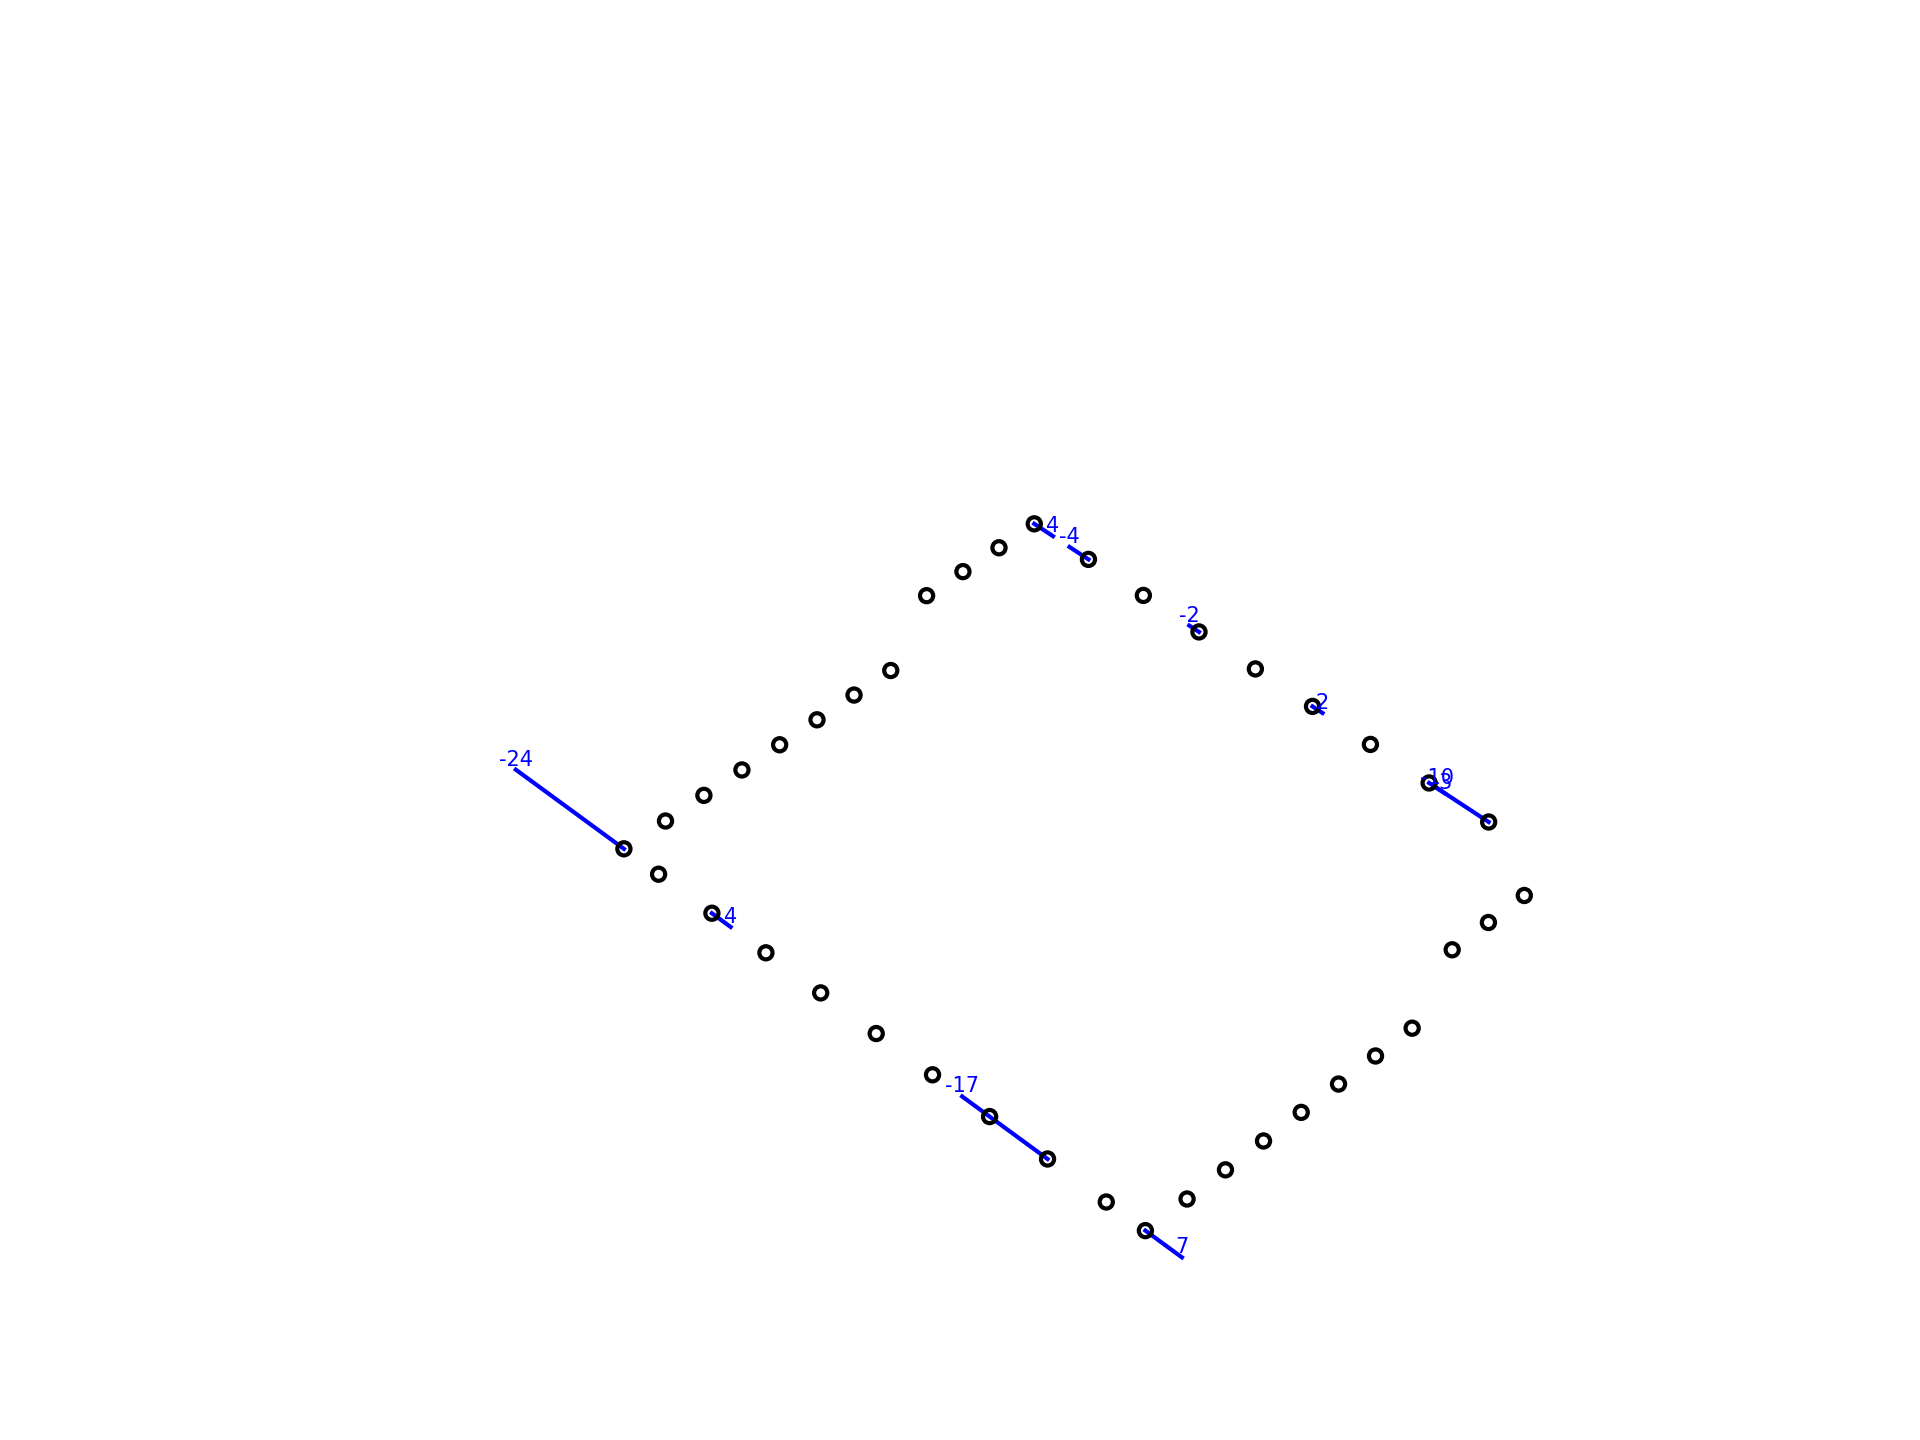
\includegraphics[width=\textwidth]{assets/img/graph3D_charges_cas_5_RFy_kN.png} % Pour insérer l'image
        \caption{max(G,S)\_RFy\_kN} % Légende de l'image
    \end{figure}

    \begin{figure}[H] % Pour insérer une figure
        \centering % Pour centrer l'image
        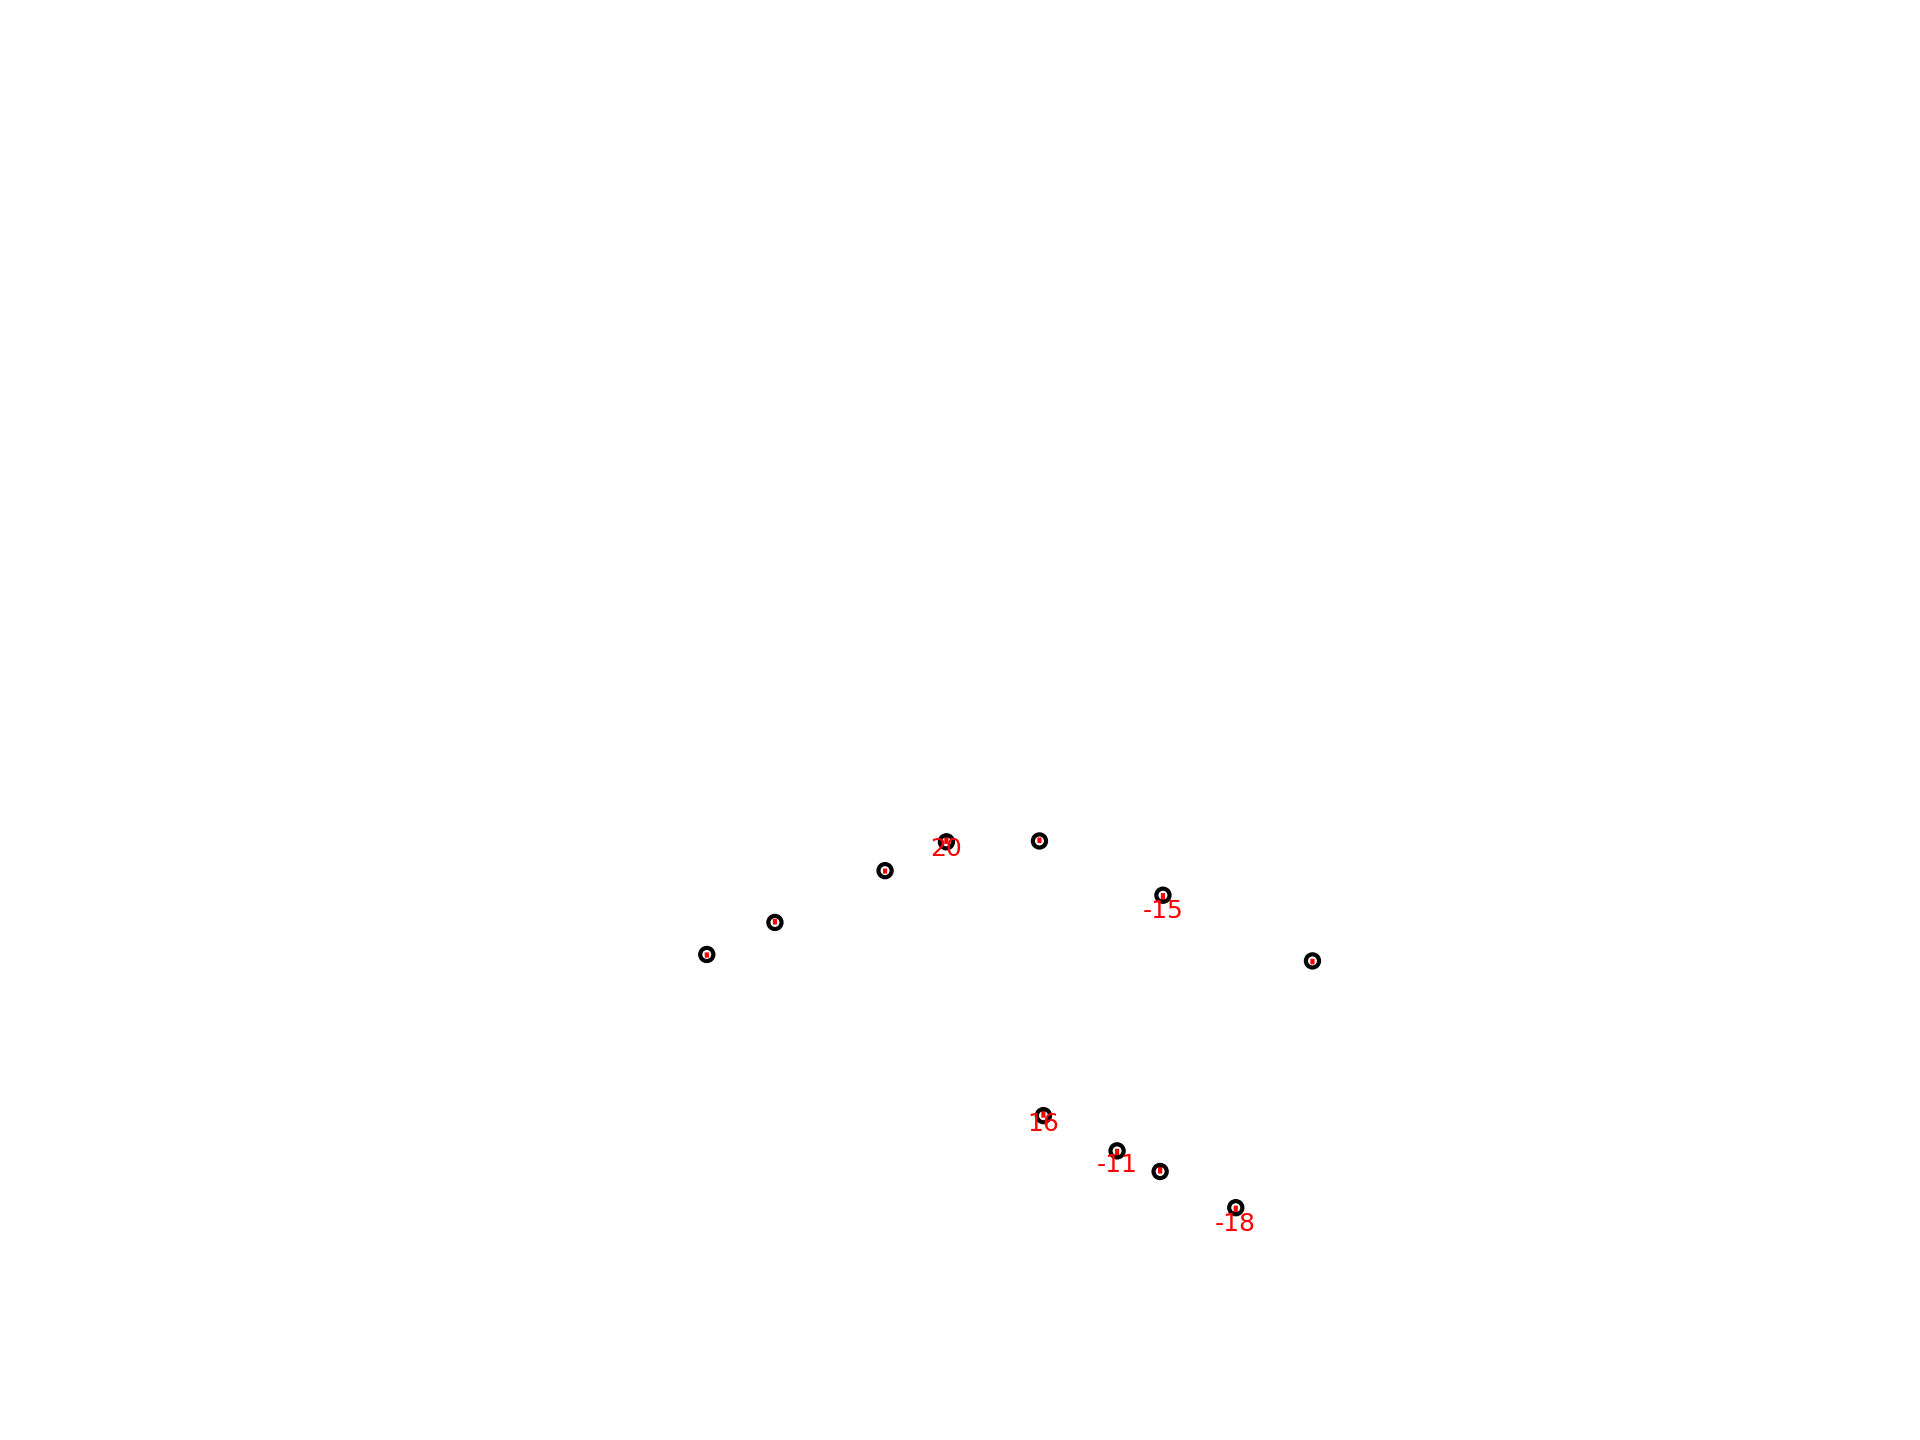
\includegraphics[width=\textwidth]{assets/img/graph3D_charges_cas_5_RFz_kN.png} % Pour insérer l'image
        \caption{max(G,S)\_RFz\_kN} % Légende de l'image
    \end{figure}

    